\section{Results}
\subsection{A quadratic problem}
To see how gradient descent works in real time, several examples will be discussed. First the function $f$ previously presented in \eqref{eq:10} will be considered. As can be seen in Figure \ref{fig:ellipsoid_3D}, $f$ attains a global minimum at $x = (0,0).$ Thus, $f$ is clearly convex. In order to verify the convexity of $f$ algebraically, Lemma \ref{second-ord-cond} will be used. The second partial derivatives of $f$ compute to: $f_{11}(x) = 1$, $f_{22}(x) = 10$ and $f_{12}(x) = 0.$ Therefore, its Hessian is given by: $
\mathcal{H} = 
\begin{bmatrix}
1 & 0 \\
0 & 10 
\end{bmatrix}
$.
We fix $x \in \mathbb{R}^{2}=\textbf{dom} (f).$ Then $x^{T} \mathcal{H} x = (x_{1}, x_{2}) \mathcal{H}  
\begin{pmatrix}
    x_{1} \\
    x_{2} 
\end{pmatrix}
= x_{1}^{2} + 10x_{2}^{2} \geq 0.
$
Since $x$ was arbitrarily fixed, the inequality holds $\forall x \in \mathbb{R}^{2} = \textbf{dom} (f).$ Therefore, $\mathcal{H}$ is positive semidefinite. Then by Lemma \ref{second-ord-cond}, $f$ is convex.
\subsubsection{Gradient descent with fixed step size}
The first observation is that $f$ is $\alpha$-strongly convex with $\alpha=1$, since $\mathcal{H} - I = \begin{bmatrix}
0 & 0 \\
0 & 9
\end{bmatrix}$ is positive semidefinite. This holds by Theorem \ref{SPD_e}, as all the eigenvalues of $\mathcal{H} - I$ are non-negative. Also, $\mathcal{H}^{T}\mathcal{H} = \mathcal{H}^{2}= \begin{bmatrix}
1 & 0 \\
0 & 100
\end{bmatrix}$.
The spectral norm of $\mathcal{H}$ is $\vertiii{\mathcal{H}}_{2} = \sqrt{100} = 10.$ Then by Remark \ref{findL}, $f$ has Lipschitz continuous gradient with $L=10.$ By the results obtained from the convergence analysis of gradient descent, choosing the step size $\tau$ such that $\tau \leq \max\{2\alpha / L^{2},\text{ } 2/(\alpha+L)\} = \max\{1/50,\text{ } 2/11\} = 2/11$ ensures convergence. We choose the starting vector to be $x^{(0)}=(10,2)$ and the stopping criterion to be $\eta = 10^{-7}.$ The situation will be analyzed for values of $\tau \in \{\frac{2}{11}, \frac{1}{11}, \frac{1}{22}, \frac{1}{44}\}.$ The algorithm computes a minimizing sequence consisting of $N$ vectors. Including the starting vector, this sequence will be: $(x^{(0)},\ldots,x^{(N)}).$ The function values evaluated at these vectors decrease iteration after iteration and get closer to the exact global minimum. For each $\tau,$ the value of interest is $N$, which denotes the total number of iterations until the the algorithm terminates. This happens, once the stopping criterion is reached, i.e.,  $||\nabla f(x)||_{2} \leq \eta$. It is important to realize that in this particular problem, the exact global minimum $p^{*}$ is known, namely when $x^{*}=(0,0),\text{ } p^{*} = f(x^{*}) = 0$. The optimality gap is the distance between the function value at the final iterate $f(x^{(N)})$ and $p^{*} = 0$ which is precisely $f(x^{(N)}).$  The convergence with the fixed step size can be visualized. Figure \ref{fig:convergence1_fixed} shows the convergence of $f(x^{(k)})$ towards the global minimum $f(x^{*})$ as the number of iterations $k$ increase, for different step sizes $\tau$.\footnote{Refer to Notebook 1, cell 7, in GitHub \cite{ThesisCode2023} for the code to create the plots and table.}
\begin{figure}[h!]
    \centering
        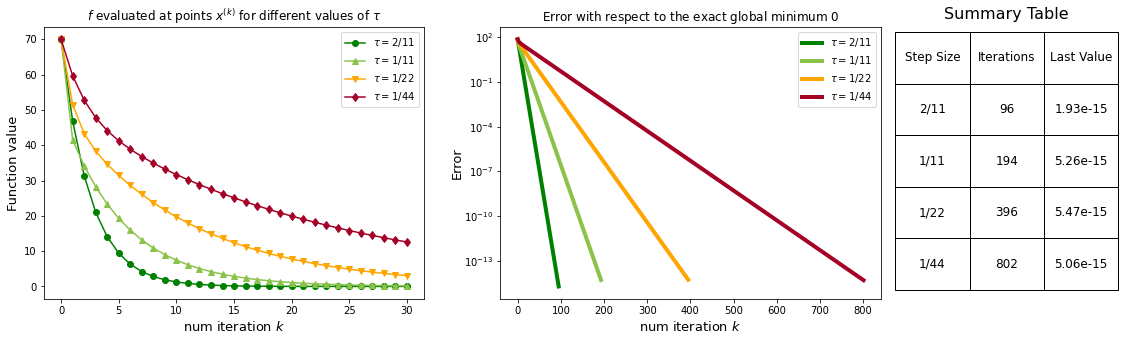
\includegraphics[width=1\textwidth]{Pictures/Merged_conv_ellipsoid_fixed_table.png}
    \caption{The left plot illustrates the convergence, while the middle plot shows the logarithmic error $f(x^{(k)})$ at each iteration up to the final iteration. On the right, a table summarizes the step sizes used, the total number of iterations, and the optimality gap.}\label{fig:convergence1_fixed}
\end{figure}\\
From the plots and the table in Figure \ref{fig:convergence1_fixed}, it can be concluded that a step size of $\tau=\frac{2}{11}$ ensures the fastest convergence among the other step sizes in $\{\frac{2}{11}, \frac{1}{11}, \frac{1}{22}, \frac{1}{44}\},$ since the number of iterations for $\tau=\frac{2}{11}$ is 96, which is substantially lower than the number of iterations for the other step sizes. Furthermore, it can be said that for each step size, the algorithm achieves a good approximation of the exact global minimum, namely one of order of magnitude of $10^{-15} (\approx 0).$   
\newpage
In order to visualize the convergence more effectively, contour plots can be very useful. A contour plot is a type of graph that shows how a function of two variables changes across different values. It does this by plotting contour lines, which are lines that connect points with the same value of the function. These contour lines help us visualize how the value of the function changes as we move around the graph. This can be particularly helpful for seeing how the gradient descent iterates $x^{(k)}$ are progressing towards the optimal solution.
The convergence can be visualized for different step sizes $\tau$. Let's choose $\tau_1 = 1/51$ and $\tau_2 = 2/11$. For step size $\tau_1$, gradient descent computes a minimizing sequence consisting of 930 vectors, and for $\tau_2$, as can be seen in the summary table in Figure \ref{fig:convergence1_fixed}, it computes a minimizing sequence consisting of 96 vectors. Figure \ref{fig:levelsets1_fixed} demonstrates the convergence for both step sizes by plotting the starting point $x^{(0)}=(10, 2),$ the two minimizing sequences and the contour lines of $f.$\footnote{Refer to Notebook 1, cell 11, in GitHub \cite{ThesisCode2023} for the code to create the contour plot.}
\begin{figure}[h!]
    \centering
        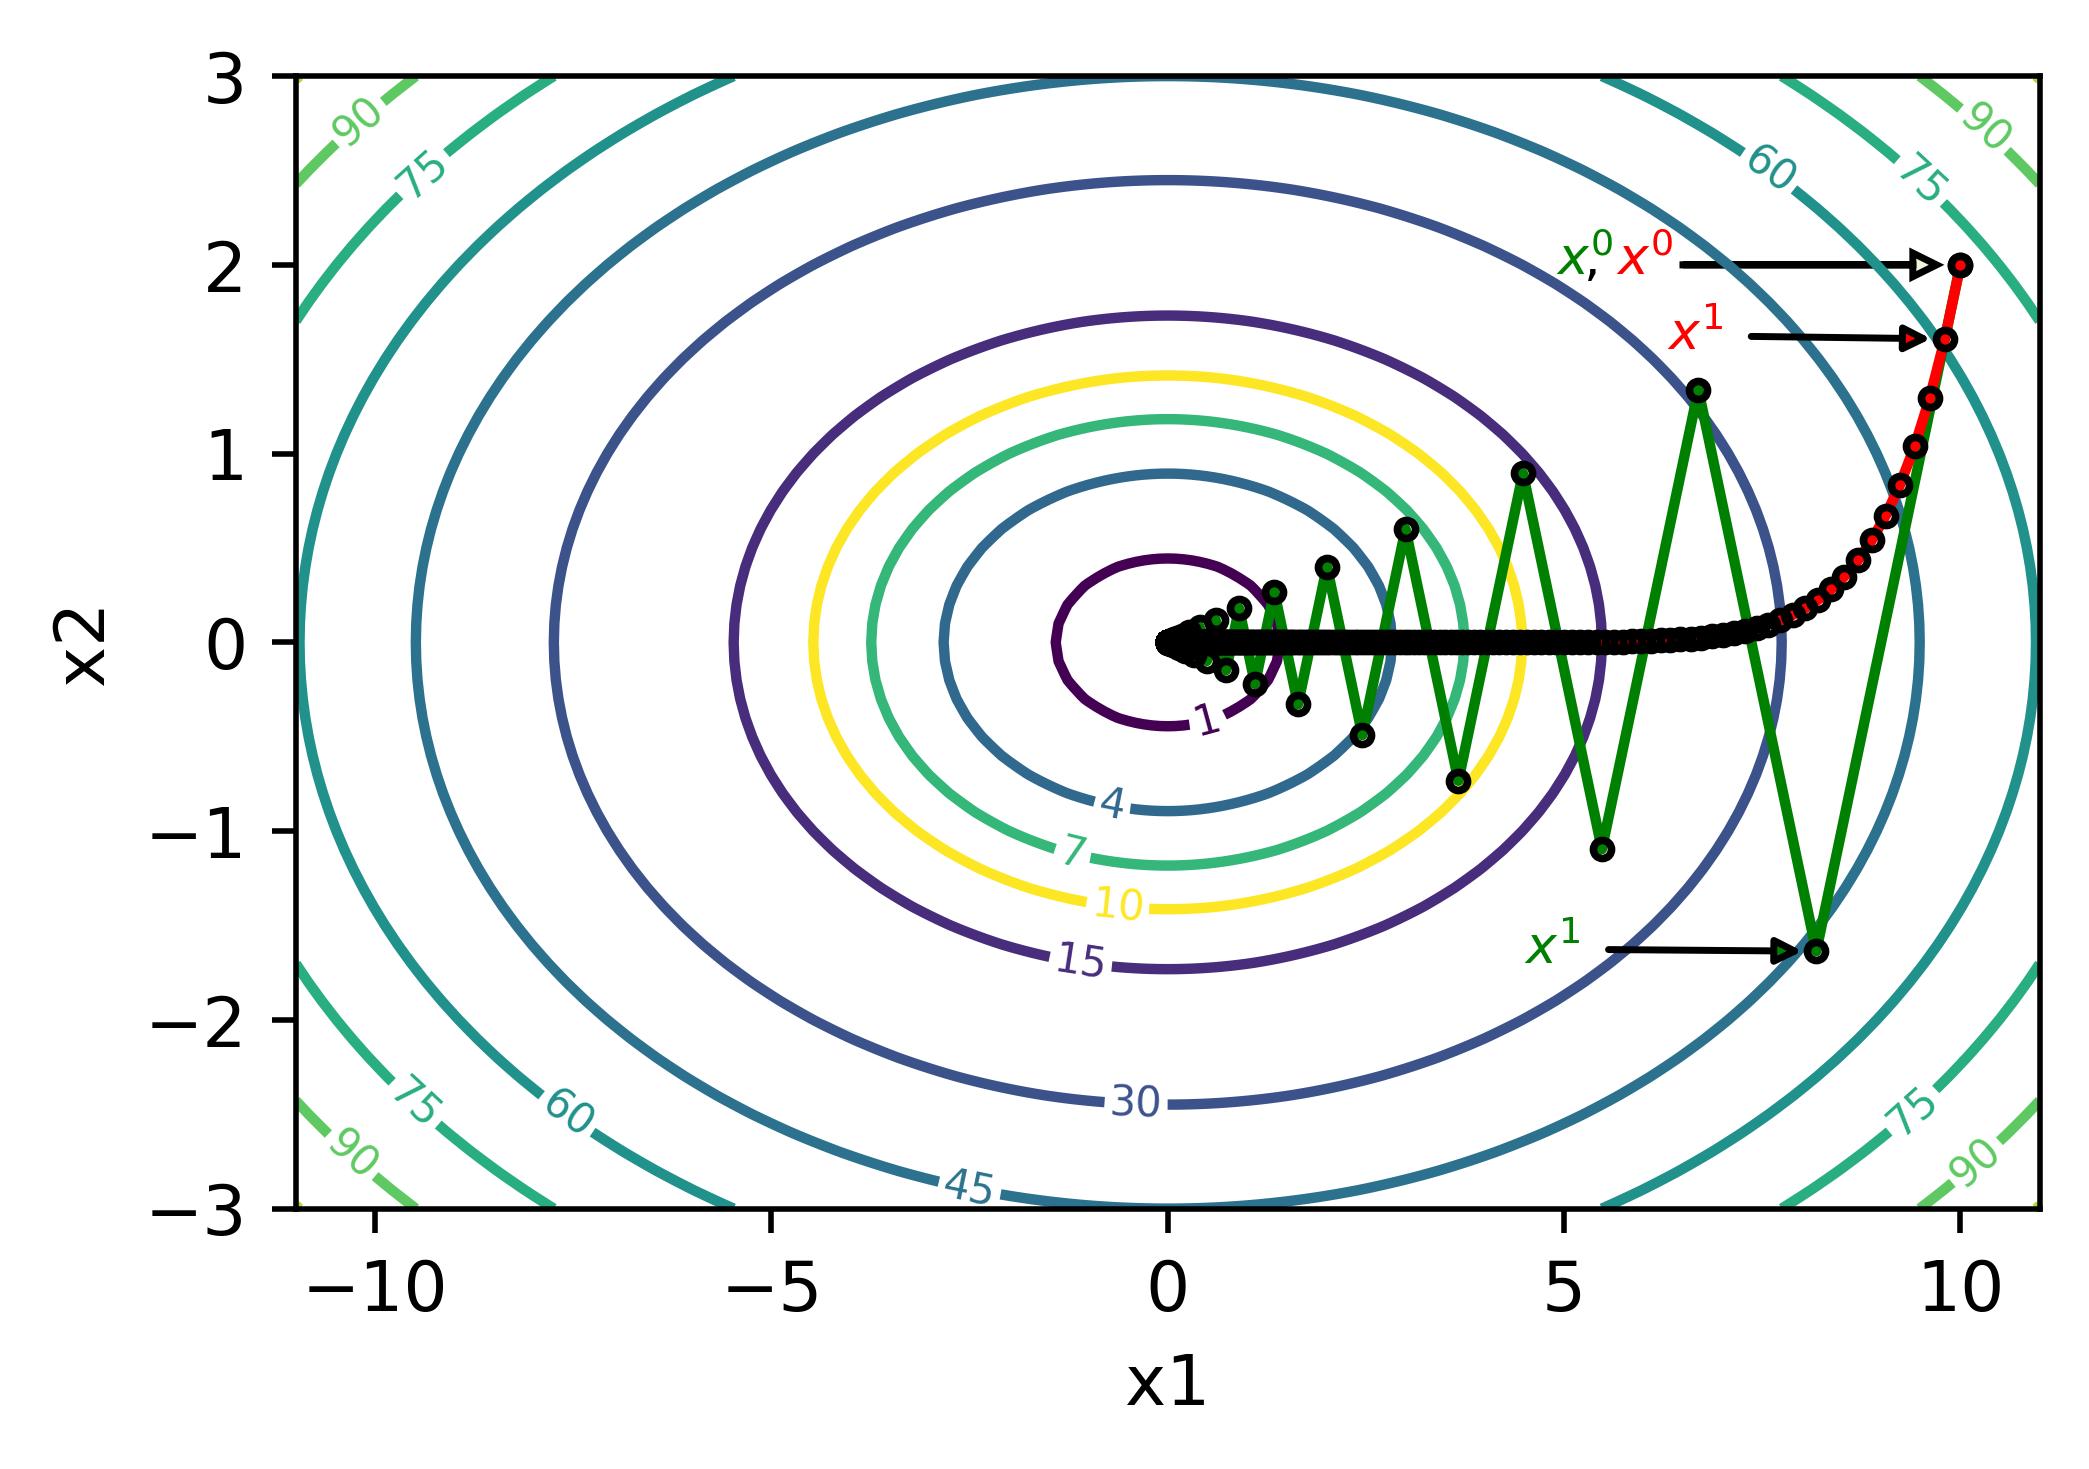
\includegraphics[width=0.58\textwidth]{Pictures/Level sets of ellipsoid_fixed.png}
    \caption{The color red represents the convergence with step size $\tau_{1}$ and green represents the convergence with step size $\tau_{2}.$ With step size $\tau_{2}$, the convergence is substantially faster than with step size $\tau_{1}.$ For the sake of illustration $\tau_{1}$ was chosen to be compared to $\tau_{2}$, since $\tau_{1}$ satisfies the bound provided by \ref{pf_gd_sc_L}.}\label{fig:levelsets1_fixed}
\end{figure}\\
It is important to note that choosing a bound larger than $\tau_{2} = 2/11$ can lead to complications. If we ignore both conditions, $\tau \leq 2/(\alpha + L)$ and $\tau < 2\alpha / L^{2}$, there's an increased likelihood of the algorithm to diverge by overshooting the minimum. In fact, attempting to apply the algorithm with a step size slightly larger than $\tau_{2}$, will result in numerical overflow (i.e., the algorithm will diverge). Figure \ref{fig:GD_ell_fixed_iter} shows the relation between the number of iterations until the algorithm terminates and the step size.\footnote{Refer to Notebook 1, cell 12, in GitHub \cite{ThesisCode2023} for the code to create the plot.} 
\begin{figure}[h!]
    \centering
        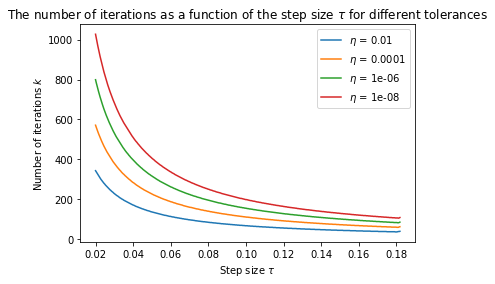
\includegraphics[width=0.65\textwidth]{Pictures/GD ellipsoid_fixed_iterations_vs_stepsize.png}
    \caption{As long as $\tau$ remains within the appropriate range, an increase in $\tau$ leads to faster convergence towards the global minimum, and hence a reduction in the number of iterations required for termination. Additionally, a looser tolerance $\eta$ results in faster convergence.}\label{fig:GD_ell_fixed_iter}
\end{figure}
\subsubsection{Gradient descent with backtracking line search} Gradient descent using backtracking line search with $\alpha = 0.3$, $\beta = 0.8$ and $\eta = 10^{-7}$ is implemented on the quadratic function $f$.\footnote{Refer to Notebook 2 in GitHub \cite{ThesisCode2023} for the implementation of GD with backtracking line search on $f.$} The number of iterations until the algorithm terminates is 92. So the algorithm computes a minimizing sequence that consists of 93 vectors: $(x^{(0)},\ldots,x^{(92)})$. The convergence of gradient descent to the exact global minimum $p^{*}=0$ with backtracking line search, can be visualized.\footnote{Refer to Notebook 2, cells 4 and 5, in GitHub \cite{ThesisCode2023} for the code to create the convergence plots.} The optimality gap is the distance between $f(x^{(92)}) = 3.5\cdot 10^{-15}$ and $p^{*}=0$ which is precisely $f(x^{(92)}).$ In Figure \ref{fig:convergence1}, on the left you can see an illustration of the convergence to $p^{*}=0$ and on the right the error $f(x^{(k)})$ with respect to $p^{*}=0$ for every $k$ up until and including 30.
\begin{figure}[h!]
    \centering
        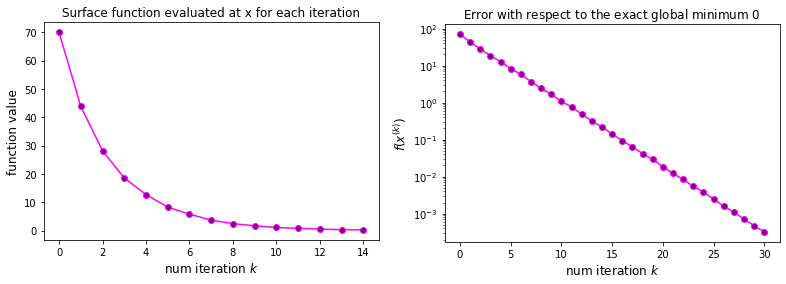
\includegraphics[width=0.85\textwidth]{Pictures/Merged_conv_ellipsoid.png}
    \caption{The left plot illustrates the convergence, while the right plot shows the logarithmic error $f(x^{(k)})$ for each $k$ up until and including 30.}\label{fig:convergence1}
\end{figure}\\
Figure \ref{fig:levelsets1} is a contour plot of $f$ showing the convergence of $x^{(k)}$ towards $x^{*}$ as k increases.\footnote{Refer to Notebook 2, cell 9, in GitHub \cite{ThesisCode2023} for the code to create the contour plot.}
\begin{figure}[h!]
    \centering
        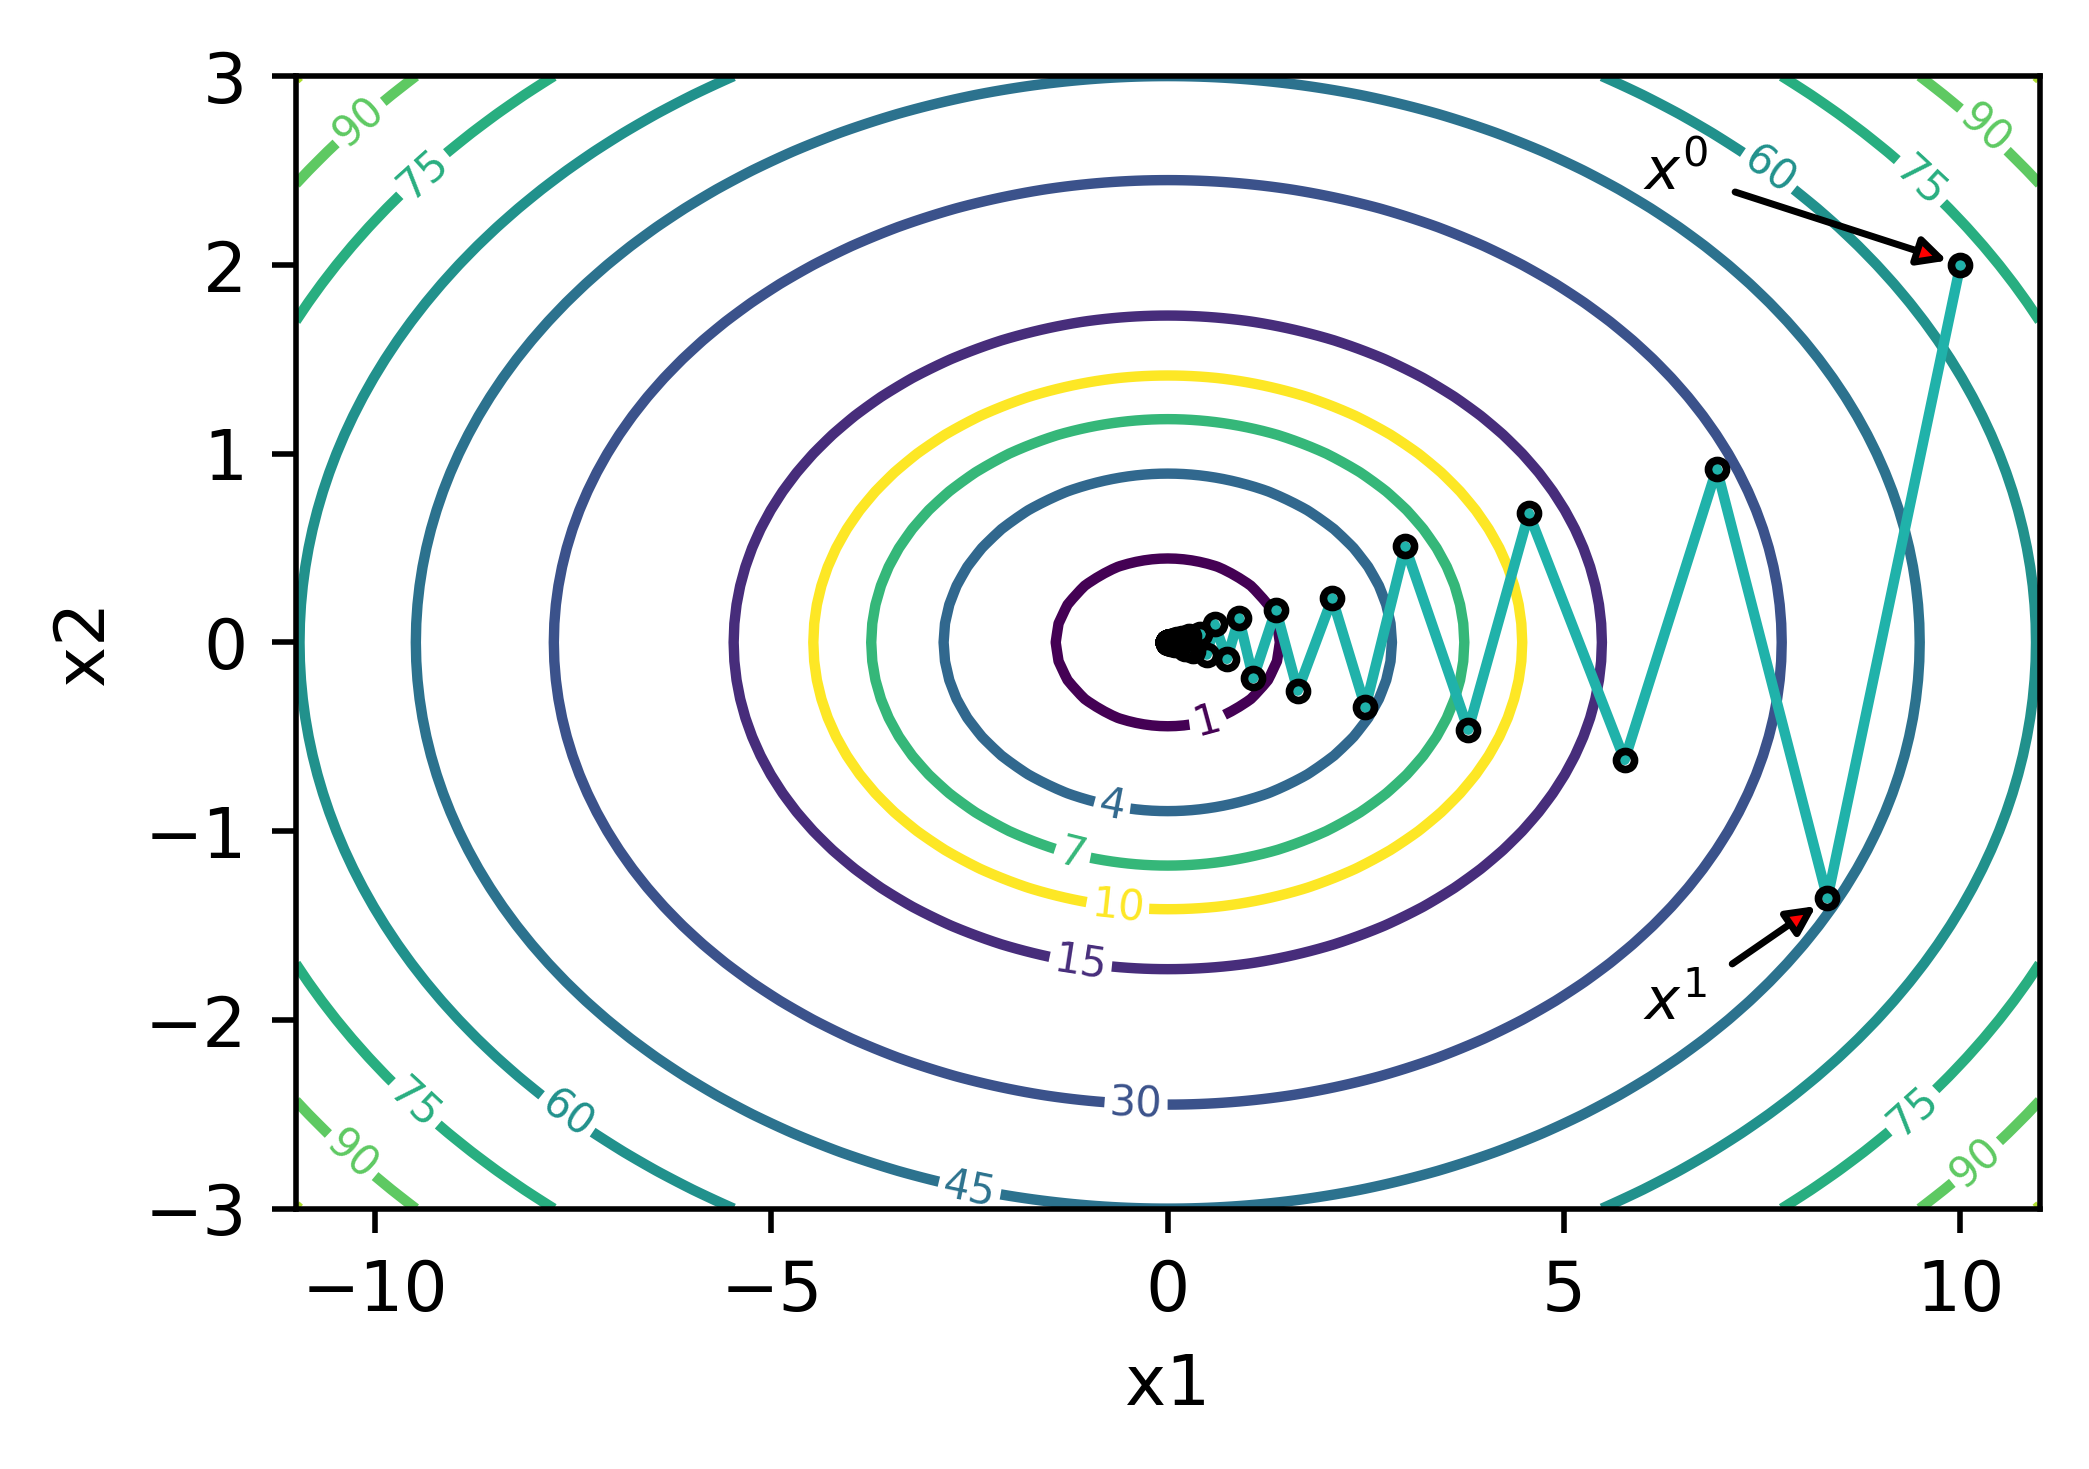
\includegraphics[width=0.58\textwidth]{Pictures/Level sets of ellipsoid.png}
    \caption{This plot shows the contour lines of the quadratic function $f,$ the points $(x^{(0)},\ldots,x^{(92)})$ and how $x^{(k)}$ gets closer to $x^{*}$ as $k$ goes from 0 to 92.}\label{fig:levelsets1}
\end{figure}\\
From these results, we observe that gradient descent with backtracking line search outperforms its counterpart with a fixed step size. The iteration count achieved here, $N=92$, is lower than all counts obtained from the fixed step size method (as shown in the table in Figure \ref{fig:convergence1_fixed}). The only iteration count that approaches this low value is $96$, which was achieved with the largest possible step size, $\tau=2/11$.
\newpage
\subsection{A non-quadratic problem}
We now consider a non-quadratic example in $\mathbb{R}^2$,  with 
\begin{equation*}\label{eq:12}\tag{6.2.1}
\begin{aligned}  
    &g(x) = e^{x_{1}+3x_{2}-0.1}+e^{x_{1}-3x_{2}-0.1}+e^{-x_{1}-0.1}
\end{aligned}
\end{equation*}
First it should be checked whether this function is convex. $g(x) = g_{1}(x)  + g_{2}(x) + g_{3}(x).$ Define: $f: y \mapsto e^{y}$. Then $g_{i}(x) = f(h_{i}(x))$ for $i=1,2,3$ and $g(x) = f(h_{1}(x)) + f(h_{2}(x)) + f(h_{3}(x)),$ where $h_{1}: x \mapsto x_{1} + 3x_{2}-0.1$, $h_{2}: x \mapsto x_{1} - 3x_{2}-0.1$, and $h_{3}: x \mapsto -x_{1}-0.1$. Since $f"(y) = e^{y} > 0 \text{ }$ for all $y \in \mathbb{R},$ $f$ is convex by Lemma \ref{second-ord-cond}. Furthermore $h_{1}, h_{2}, h_{3}$ are affine. By Definition \ref{compaf} the composition of a convex function with an affine function is convex, so $g_{i}(x) = f(h_{i}(x))$ is convex for $i=1,2,3.$ The sum of convex functions is also convex, therefore $g$ is convex. Figure \ref{fig:exp} is a 3D plot of $g.$\footnote{Refer to Notebook 6, cell 6, in GitHub \cite{ThesisCode2023} for code details.}
\begin{figure}[h!]
    \centering
        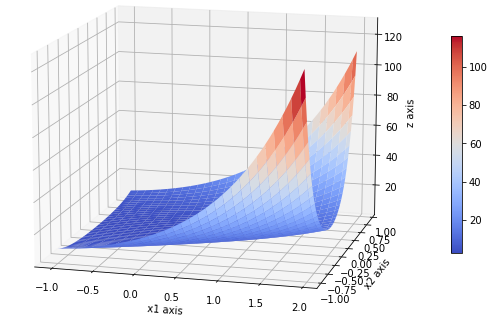
\includegraphics[width=0.36\textwidth]{Pictures/3D plot of an exponential function.png}
    \caption{3D surface plot of the function $g$}\label{fig:exp}
\end{figure}\\
Gradient descent with backtracking line search and parameters $\alpha = 0.1$, $\beta = 0.7$ and stopping criterion $\eta = 10^{-7}$ is implemented on the non-quadratic function $g$.\footnote{Refer to Notebook 3 in GitHub \cite{ThesisCode2023} for the implementation of GD with backtracking line search on $g.$} We choose the starting vector to be $x^{(0)} = (-1,0.5)$. The algorithm computes a minimizing sequence of 39 vectors. Together with the starting vector we find the sequence: $(x^{(0)},\ldots,x^{(39)}).$ The function value decreases iteration after iteration and whenever $||\nabla f(x)||_{2} \leq \eta$, the algorithm terminates. The figure below shows the convergence to the global minimum $g(x^{*}) \approx g(x^{(39)})=2.559$, where the plot on the left is an illustration of the convergence to $g(x^{*})$ and the plot on the right the error $g(x^{(k)}) - g(x^{(39)})$ for every $k$ up until and including 39.\footnote{Refer to Notebook 3, cells 4 and 5, in GitHub \cite{ThesisCode2023} for the code to create the convergence plots.} 
\begin{figure}[h!]
    \centering
        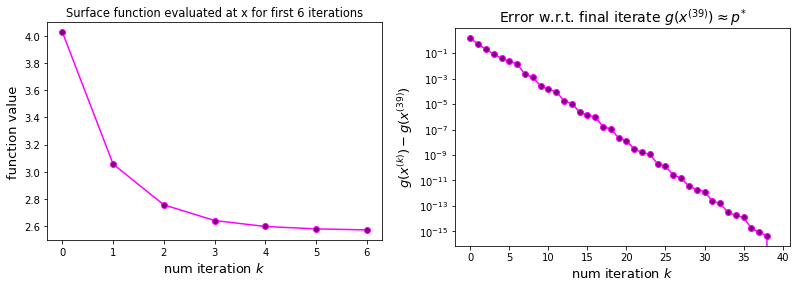
\includegraphics[width=0.7\textwidth]{Pictures/Merged_conv_exponential.png}
    \label{fig:convergence2}
\end{figure}\\
Similar to the quadratic function $f$, a contour plot can also be provided for $g.$ The contour lines of the non-quadratic function $g$ and the points $(x^{(0)},\ldots,x^{(39)})$ are shown in the figure below.\footnote{Refer to Notebook 3, cell 9, in GitHub \cite{ThesisCode2023} for the code to create the contour plot.}
\begin{figure}[h!]
    \centering
        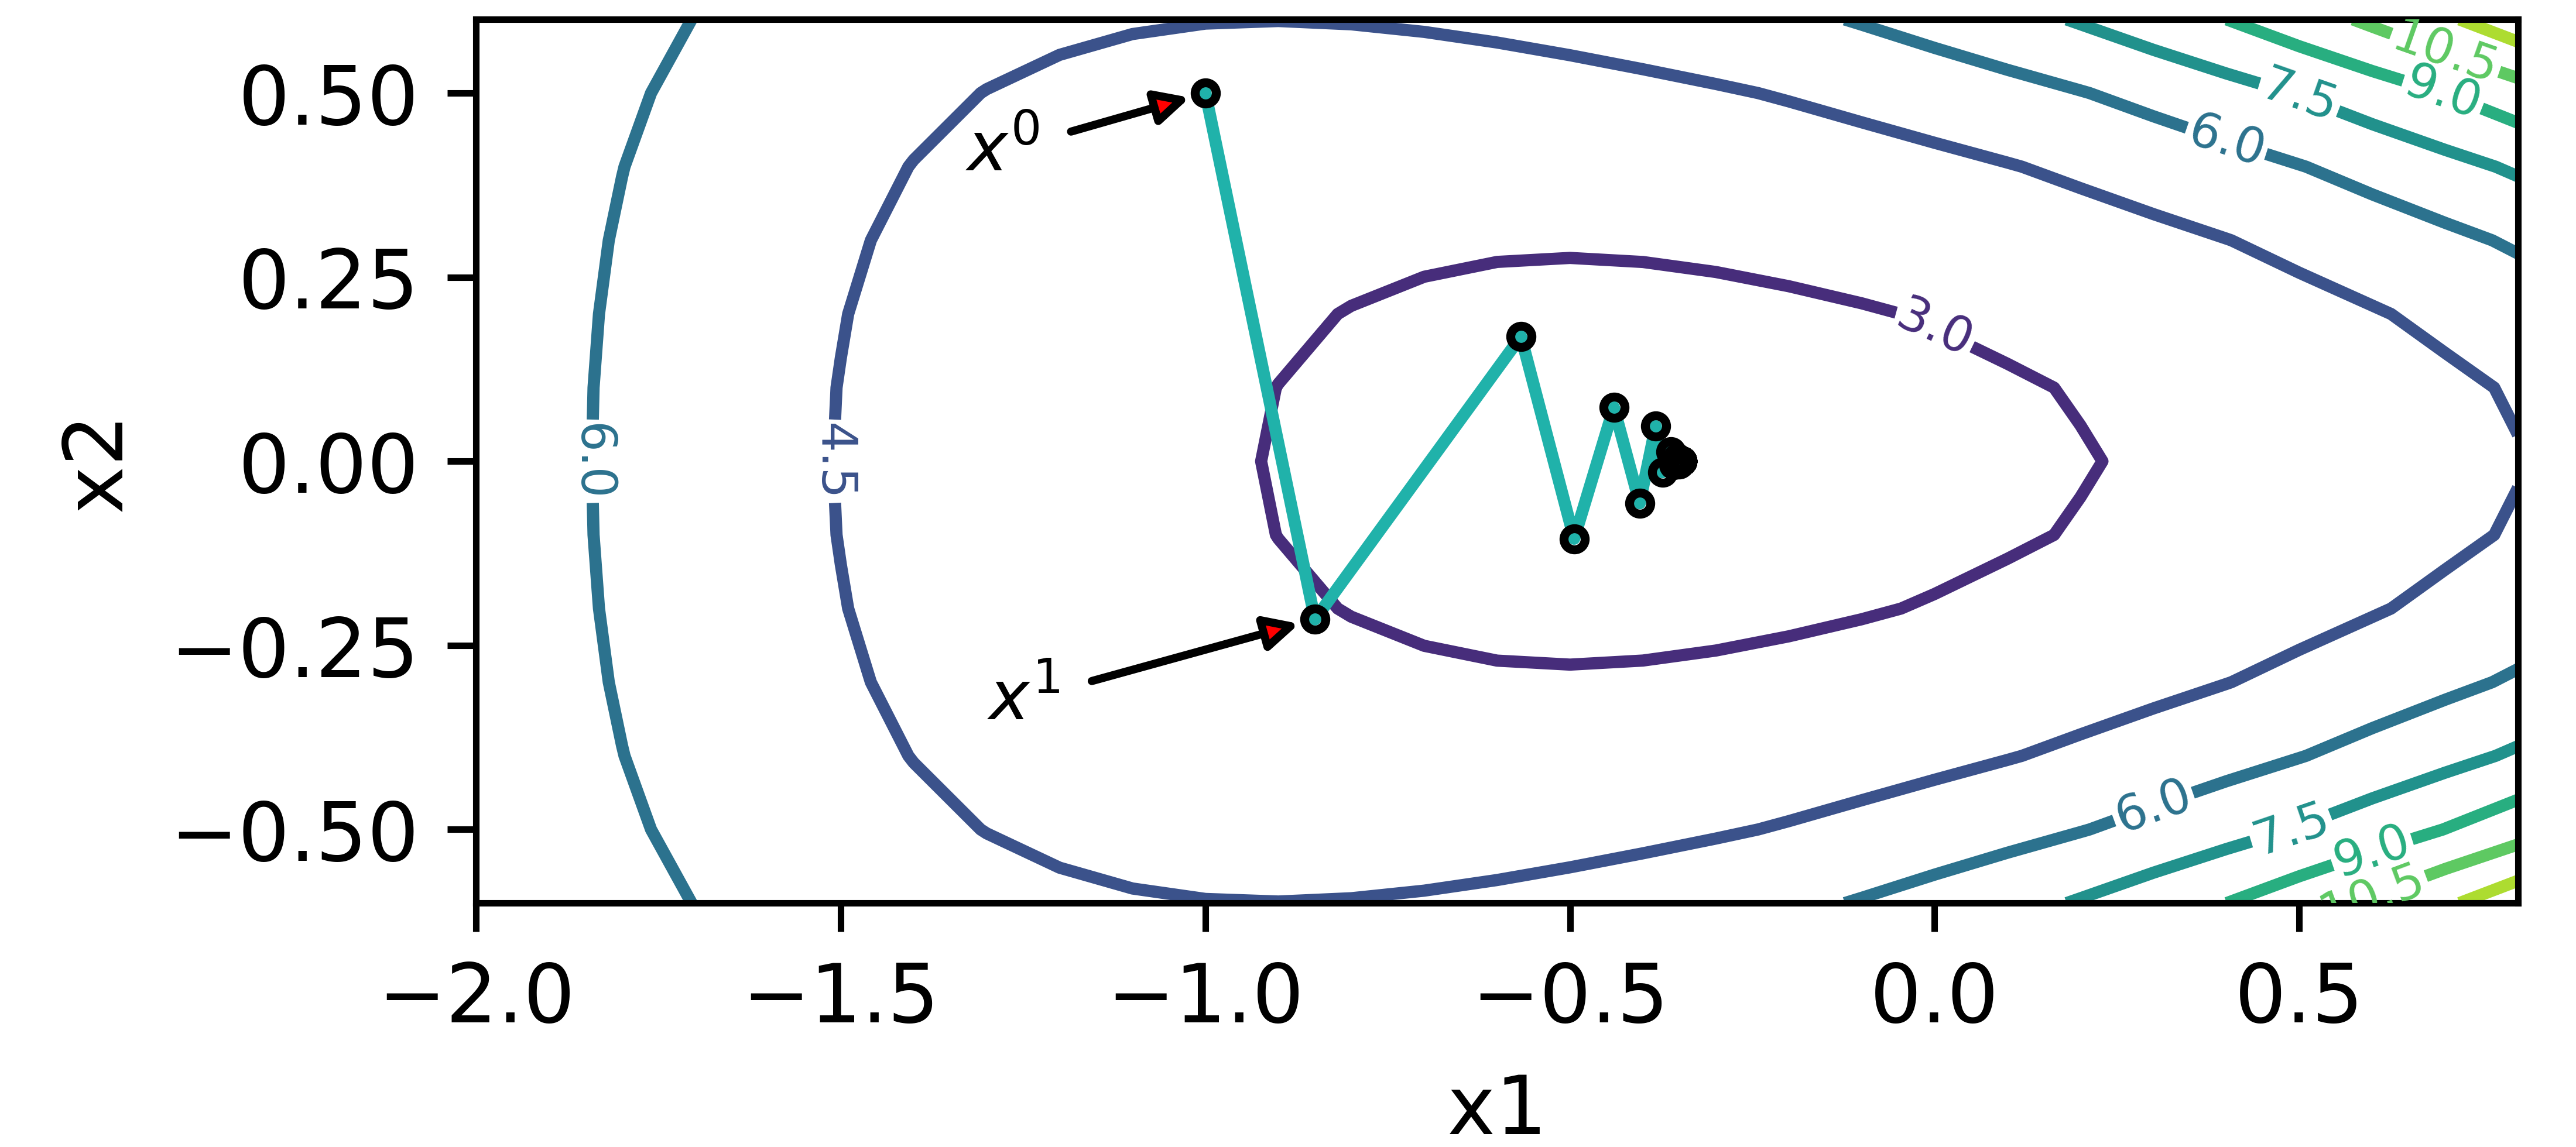
\includegraphics[width=0.525\textwidth]{Pictures/Level sets of exponential.png}
    \label{fig:levelsets2}
\end{figure}\\
\newpage
\subsection{A multi-dimensional non-convex problem}
We now aim to minimize Ackley's function, which is expressed in Formula \eqref{eq:18}. This function is widely used for testing optimization algorithms \cite{Test_functions}. In its two-dimensional form, as shown in Figure \ref{fig:Ackelys_plot}, it is characterized by a nearly flat outer region, and a large hole at the centre.\footnote{Refer to Notebook 6, cells 7 and 8, in GitHub \cite{ThesisCode2023} for the code to create 3D plots of Ackley's function.}
\begin{equation*}\label{eq:18}\tag{6.3.1}
\begin{aligned}
&h(x) = -a\exp\left(-b\sqrt{\frac{1}{d}\sum_{i=1}^{d} x_{i}^{2}}\right) - \exp\left(\frac{1}{d}\sum_{i=1}^{d} \cos(cx_{i})\right) + a + \exp(1) 
\end{aligned}
\end{equation*}
\begin{figure}[h!]
    \centering
        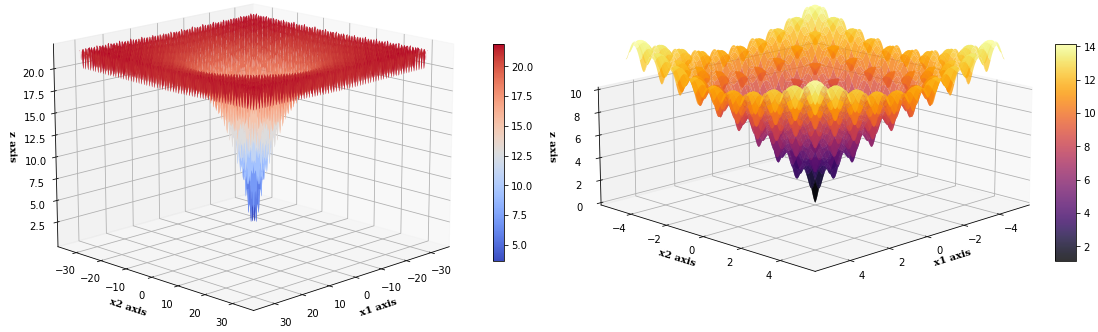
\includegraphics[width=0.85\textwidth]{Pictures/Merged_Ackleys_plot.png}
    \caption{3D plots of $h$ on $x_{i} \in [-32.768,\text{ } 32.768]$, and on $x_{i} \in [-5,\text{ } 5]$}\label{fig:Ackelys_plot}
\end{figure}\\
In machine learning, many cost functions are non-convex. $h$ is an example of a non-convex function that is also multimodal, i.e., it has multiple local minima. This possesses a risk for gradient-based optimization methods, since they can become trapped in one of the local minima and thus fail to find the global minimum. Although Ackley's function is a better benchmark function to test global optimization methods like simulated annealing and particle swarm optimization, the performance of gradient-based methods will also be assessed to demonstrate the potential challenges. The global minimum of $h$ is known, namely when $x^{*} = 0,$ we have $h(x^{*}) = 0.$ 
\subsubsection{Gradient descent with backtracking line search} Consider $h$ with dimension $d=100.$ For the variable values take: $a = 20,\text{ }b = 0.2,$ and $c = 2\pi$. Gradient descent using backtracking line search with $\alpha = 0.1, \beta = 0.8$ and stopping criterion $\eta = 10^{-6}$ is implemented on $h.$\footnote{Refer to Notebook 4 in GitHub \cite{ThesisCode2023} for the implementation of GD with backtracking line search on $h.$} To test convergence, a vector $x^{(0)}$ is created randomly such that each term lies in $[-32.768, 32.768]$.\footnote{Download 'input.npy' from GitHub \cite{ThesisCode2023} and refer to Notebook 4, cell 4 for the code to load the random vector.} Secondly, the algorithm is tested by choosing a starting vector that is close to the origin, namely $x^{(0)}=(0.4,\ldots,0.4).$ Figure \ref{fig:Ackelys_conv_check} shows the progression of the algorithm for the two different starting vectors.\footnote{Refer to Notebook 6, cell 5, in GitHub \cite{ThesisCode2023}  for the code to create the convergence plots.}
\begin{figure}[h!]
    \centering
        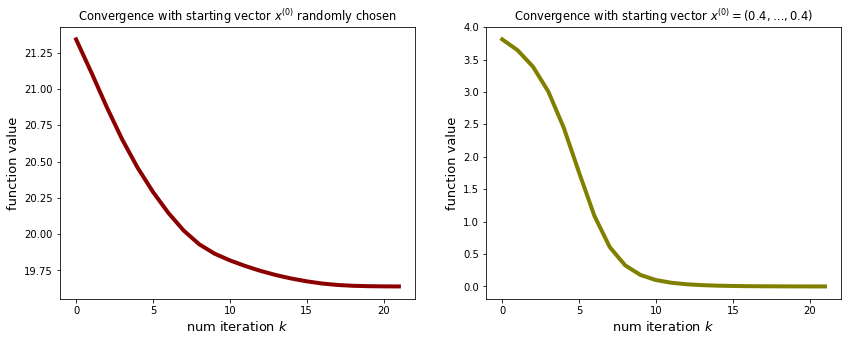
\includegraphics[width=0.75\textwidth]{Pictures/Merged_conv_ackleys.png}
    \caption{Plots to check convergence of GD for two different starting vectors.}\label{fig:Ackelys_conv_check}
\end{figure}\\
\newpage
From the results in Figure \ref{fig:Ackelys_conv_check}, the main limitation of gradient descent becomes evident: it is highly susceptible to local minima due to its inherent reliance on gradient information. For a randomly created starting vector, the function values $h(x^{(k)})$ converge towards one of the many local minima of $h$, and only if $x^{(0)}$ is chosen to be very close to the optimal solution, the values $h(x^{(k)})$ converge towards the global minimum. This experiment underscores the importance of selecting appropriate optimization methods for specific problems. A natural question is whether stochastic gradient descent (SGD) can be applied to this problem. SGD is specifically designed for objective functions that are often used in machine learning, which typically involve large datasets. However, $h$ is a mathematical function that does not have the desirable form of a sum of functions. Consequently, there is no natural way to divide the function into smaller subsets. In other words, the gradient information in $h$ is deterministic and does not depend on a dataset, which eliminates stochasticity from the problem and makes SGD not applicable.

\subsubsection{Simulated Annealing (SA)}
An alternative to gradient descent is simulated annealing with pseudo-code given in Algorithm \ref{Pseudocode_SA}. The problem parameters remain unchanged: $d=100, a=20, b=0.2,$ and $c=2\pi.$ The algorithm is tested for two different starting vectors, namely one that is randomly generated with terms lying in $\left[-32.768,32.768\right]$ and one that is closer to the optimal solution with terms in $\left[-5,5\right].$ The initial temperature is chosen to be $t_0=5.0$ and cooling schedule $t_{k} = 0.99^{k}t_0.$ The algorithm terminates when the maximum number of iterations $k_{max}=400$ is reached. Figures \ref{fig:SA_conv1} and \ref{fig:SA_conv2} illustrate the possible paths the algorithm can take for the values $h(x^{(k)})$ to progress towards the global minimum. In the left figure, the algorithm converges for both starting vectors, whereas the right figure shows a scenario in which the algorithm for one of the starting vectors gets trapped in a local minimum of $h$.\footnote{Refer to Notebook 5, cell 2, in GitHub \cite{ThesisCode2023} for the code to create paths similar to the ones in Figures \ref{fig:SA_conv1} and \ref{fig:SA_conv2}.}
\begin{figure}[h]
  \centering
  \begin{minipage}[b]{0.3387\textwidth}
    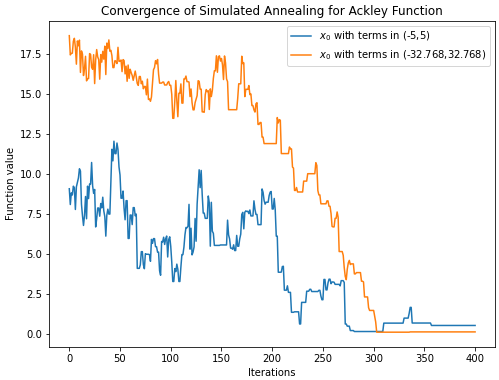
\includegraphics[width=\textwidth]{Pictures/sa_convergence-ackley3-38-c.png}
    \caption{Example 1}\label{fig:SA_conv1}
  \end{minipage}
  \hspace{0.05cm} 
  \begin{minipage}[b]{0.33\textwidth}
    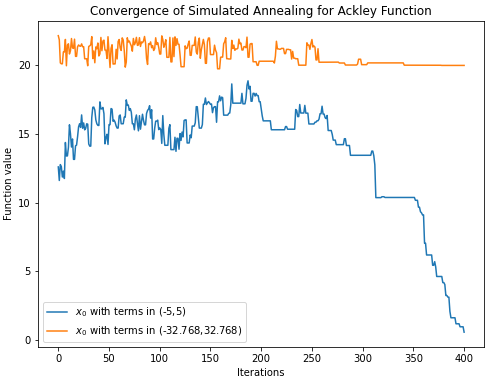
\includegraphics[width=\textwidth]{Pictures/sa_convergence-ackley3-37_c.png}
    \caption{Example 2}\label{fig:SA_conv2}
  \end{minipage}
\end{figure}\\
In order to visualize the stochasticity in the algorithm, we consider $h$ with dimension $d=2.$ In this setting, contour plots of $h$ and the progression of $h(x^{(k)})$ towards possibly the global minimum can be plotted. Figures \ref{fig:SA_cont1} and \ref{fig:SA_cont2} below illustrate the progression of simulated annealing for two different starting vectors in $\mathbb{R}^2$ with terms in $\left[-10, 10\right].$\footnote{Refer to Notebook 5, cell 3, in GitHub \cite{ThesisCode2023} for the code to create contour plots similar to the ones in Figures \ref{fig:SA_cont1} and \ref{fig:SA_cont2}.}
\begin{figure}[h]
    \centering
    \begin{minipage}[b][0.36\textwidth]{0.34\textwidth}
      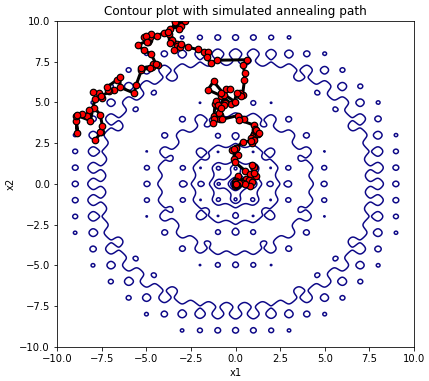
\includegraphics[width=\textwidth]{Pictures/sa_convergence-ackley_contour11.png}
      \caption{Example 1}\label{fig:SA_cont1}
    \end{minipage}
    \hspace{0.05cm}
    \begin{minipage}[b][0.36\textwidth]{0.34\textwidth}
      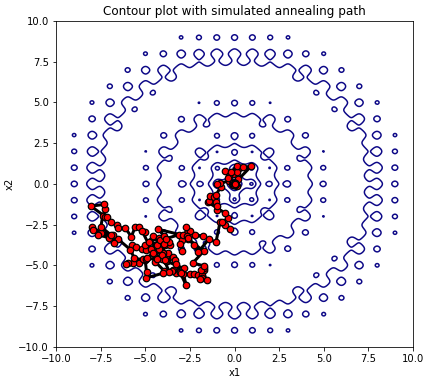
\includegraphics[width=\textwidth]{Pictures/sa_convergence-ackley_contour18.png}
      \caption{Example 2}\label{fig:SA_cont2}
    \end{minipage}
\end{figure}
\subsubsection{Particle Swarm Optimization (PSO)}
As described in Section \ref{PSO_s}, Particle Swarm Optimization (PSO) is a stochastic global optimization algorithm that performs well on multi-dimensional non-convex functions. As such, it is worth applying to minimize $h$. The algorithm is implemented in Python 3.10 \cite{python} with cognitive and social constants set to $C_{1}=0.5$ and $C_{2}=0.3$, respectively, and the maximum number of iterations set to $k_{max}=2000$. The only remaining parameter to determine is the size of the swarm. It is insightful to visualize the trajectory of the best function evaluations (i.e., the lowest function values in each iteration) up until termination for different swarm sizes. Figure \ref{fig:PSOConvMultipleSwarmSizes} displays the trajectories for various swarm sizes, specifically for $N=50$, $N=200$, $N=500$, and $N=1000$. The table on the right provides the best cost (lowest function evaluation) for each of the four swarm sizes.\footnote{Refer to Notebook 5, cells 4 and 5, in GitHub \cite{ThesisCode2023} for the code to create the convergence plot and table.}
\begin{figure}[h!]
    \centering
        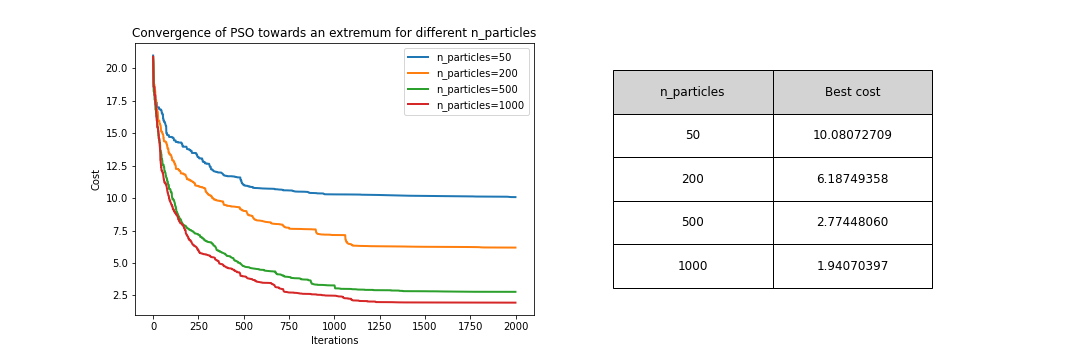
\includegraphics[width=1.12\textwidth]{Pictures/PSO_convergence-ackley_multiple_n_particles_with_table.png}
    \caption{This figure displays four trajectories of PSO distinguished by different swarm sizes n\textunderscore particles on the left and the best cost obtained for each of the cases in a table on the right.}\label{fig:PSOConvMultipleSwarmSizes}
\end{figure}\\
As can be seen from the figure, an increase in the swarm size, leads to convergence towards a minimum with a lower cost. It can also be noted, that none of the four cases reach the global minimum. This has to do with the design of the algorithm. PSO does not allow for worse function values (i.e., ones that are higher than the previous iterations), therefore it is sensitive to getting stuck in local minima. $h$ contains many local minima, and some of these local minima are very close to the global minimum. The number of local minima increases when the dimensionality of the problem increases. Since in this example, the dimension is $d=100,$ it becomes very unlikely for the swarm to collectively reach the global minimum. When $d$ is kept low, the likelihood that the algorithm succeeds in reaching the global minimum increases. To see whether this is indeed the case, PSO is performed on $h$ with $d=2.$ $C_{1}$ and $C_{2}$ remain unchanged. $k_{max}$ is set to $100$ and the size of the swarm is set to $50.$ The following figure shows the trajectory of the swarm towards the global minimum. Three different time steps are taken, namely $k=0,$ $k=10,$ and $k=100.$ For each time step a contour plot of the function and the positions of the particles are depicted in Figure \ref{fig:PSO_2D_swarm}.\footnote{Refer to Notebook 5, cell 6, in GitHub \cite{ThesisCode2023} for the code to create the particles' positions plots.}
\begin{figure}[h!]
    \centering
        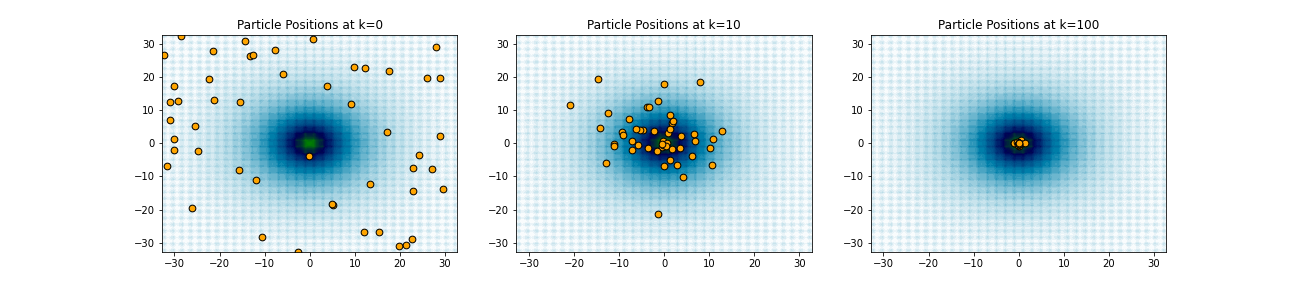
\includegraphics[width=1\textwidth]{Pictures/PSO_ackleys_2D_swarm.png}
    \caption{Contour plots and particle positions at time steps $k=0,$ $k=10,$ and $k=100$}\label{fig:PSO_2D_swarm}
\end{figure}\\
\newpage
\subsubsection{Comparison of Methods}
The effectiveness of various optimization methods was compared in minimizing Ackley's function $h$ with dimension $d=100$. First, gradient descent with backtracking line search was implemented. Before the implementation, it was anticipated that the algorithm's likelihood of finding the global minimum would be low, because Ackley's function contains numerous local minima that are closely spaced, and since gradient descent is highly sensitive to extrema, it can easily get stuck in a local minimum that isn't the global minimum. The results support this notion, as the algorithm became stuck in a local minimum when the starting vector was chosen randomly. Next, simulated annealing (SA) was implemented and found to perform quite well. In fact, it was able to locate the global minimum. The primary reason for this success is that the algorithm is designed to escape local minima easily by allowing hill-climbing moves, which temporarily worsen the function evaluation outcome, but give the algorithm time to converge towards the global minimum. Finally, particle swarm optimization (PSO) was implemented. This algorithm performed better than gradient descent by finding superior solutions, but it was still outperformed by SA, as it could not locate the global minimum. Additionally, to obtain a better solution with PSO, the swarm size had to be significantly increased, which greatly impacted computer time. In conclusion, while both SA and PSO outperformed gradient descent, they did so at the expense of more computer time.

\subsection{Application of SGD on a Neural Network}
\subsubsection{The Data}
For this application, the MNIST dataset of handwritten digits will be considered \cite{deng2012mnist}. The MNIST dataset is frequently chosen in machine learning models, due to its simplicity, which allows for an effective demonstration of experimental results. Each data point in the dataset is a pair comprising a grayscale handwritten image of a digit (28 pixels by 28 pixels) and its associated label indicating the true value of the digit. The dataset contains $N=70,000$ such data pairs. To prepare the images for input into the neural network, the 28x28 pixel image is flattened into a 1D array of 784 elements. Each element represents a grayscale value between 0 (black) and 255 (white), which are typically normalized to be a floating-point number between 0 and 1. Thus, an example input vector for the neural network would be $x^{(i)} \in \mathbb{R}^{784}$, where $i \in \{1,\ldots,n\}.$ The output vector $\hat{y}^{(i)} \in \mathbb{R}^{10}$, where $i \in \{1,\ldots,n\}$, can be interpreted as a probability distribution over the ten digit classes, 0-9. Each component of the output vector, $\hat{y}_{j}^{(i)}$, where $j \in \{1,\ldots,10\}$, represents the predicted probability that the input image corresponds to the $(j-1)$-th digit. The sum of all the terms of  $\hat{y}^{(i)}$ is 1, conforming to the properties of a probability distribution. For example, if all of the terms of the vector $\hat{y}^{(i)}$ are equal to 0.1, it would imply that the network is uncertain about the digit class of the input image, assigning an equal probability to each class. Ideally, during training, the neural network learns to confidently classify each image into one of the 10 classes, representing the digits 0-9. This means that the output vector $\hat{y}^{(i)}$ should have one entry that is significantly larger than the others, indicating a high probability for the true digit class.
\subsubsection{Neural Network Architecture (NNA) \& Training Procedure}
The neural network architecture is defined in the programming language Python 3.10 \cite{python} using the open-source deep learning framework PyTorch 2.0 \cite{NEURIPS2019_9015}. The neural network is a feed-forward neural network consisting of an input layer, two hidden layers and an output layer. The input layer, consisting of 784 neurons, corresponds to the size of the flattened input image. It is fully connected to a subsequent hidden layer that consists of 128 neurons. This layer, in turn, is fully connected to another hidden layer housing 64 neurons. The final link in this chain is a connection to the output layer, which consists of 10 neurons. So, the structure of the network is: Input(784) - Hidden1(128) - Hidden2(64) - Output(10).\footnote{Refer to Notebook 7, cells 1-4, in GitHub \cite{ThesisCode2023} for the code to define the NNA and load the data.} As discussed in Paragraph \ref{Basic_of_FFNN}, we now provide a detailed mathematical description of how the feed-forward neural network is designed and how it is trained to accurately predict the correct digit for a given input. In the neural network, the connection parameters between the layers are as follows: the input layer and the first hidden layer are interconnected through the weight matrix $W^{(1)} \in \mathbb{R}^{784 \times 128}$ and the bias vector $b^{(1)} \in \mathbb{R}^{128}$. The connection between the first and second hidden layers is established via the weight matrix $W^{(2)}\in\mathbb{R}^{128\times 64}$, alongside the bias vector $b^{(2)} \in \mathbb{R}^{64}$. Lastly, the second hidden layer and the output layer are linked through the weight matrix $W^{(3)}\in \mathbb{R}^{64\times10}$, complemented by the bias vector $b^{(3)}\in \mathbb{R}^{10}$. All these parameters are initialized before the start of the training process.
\newpage
The dataset consists of handwritten digits, $\{x^{(1)},\ldots,x^{(N)}\},$ where $N=70,000$ is the size of the dataset. This data is divided into three sets: training, validation, and testing. Out of the total $70,000$ examples, $n=54,000$, are allocated for training, $6,000$, are set aside for validation, and the remaining $10,000$ examples are used for testing. The training data, $\{x^{(1)},\ldots,x^{(n)}\},$ with $n=54,000$, is randomly shuffled and divided into a set of $M$ mini-batches of size roughly 64 data points each: $\{B_{1},\ldots,B_{M}\}.$ For each mini-batch, we have a matrix of input vectors $X \in \mathbb{R}^{m \times 784}$, where $m$ is the batch size ($\approx64$), and each row of $X$ is an input vector $x^{(i)},$ where $i \in \{1,\ldots,m\}.$
To showcase how an input vector is handled by the neural network we fix a mini-batch $B\in\{B_{1},\ldots,B_{M}\}$ and an input vector $x^{(i)}\in B.$ In the first hidden layer, a linear transformation of the form $W^{(1)^T}x^{(i)} + b^{(1)}$ is computed. Here $W^{(1)^T}x^{(i)}$ represents the dot product between each column of $W^{(1)}$ and the input vector $x^{(i)},$ where the $j$-th column of $W^{(1)}$ consists of all the weights connecting each neuron in the input layer to the $j$-th neuron in the first hidden layer $\forall j \in \{1,\ldots,128\}$. The ReLU (Rectified Linear Unit) activation function is then applied element-wise on this output, yielding $h^{(i,1)} = \text{ReLU}(W^{(1)^T}x^{(i)} + b^{(1)}),$ where $h^{(i,1)} \in \mathbb{R}^{128}.$ The ReLU activation function is a popular choice in neural networks for introducing non-linearity. It is defined as follows: 
\begin{equation*}\tag{6.4.2.1} 
\text{ReLU}(x) = \text{max}\{0, x\}, \text{ } \text{where} \text{ } \text{ReLU}:\mathbb{R} \rightarrow \mathbb{R}.
\end{equation*}
This procedure is repeated for the second hidden layer, now using $h^{(i,1)}$ as the input and applying weights $W^{(2)} \in \mathbb{R}^{128 \times 64}$ and biases $b^{(2)} \in \mathbb{R}^{64}.$
Thus, we compute $h^{(i,2)} = \text{ReLU}(W^{(2)^T}h^{(i,1)} + b^{(2)}).$

Finally, the output layer of the network performs another linear transformation, now using $h^{(i,2)}$ as the input and applying weights $W^{(3)}\in \mathbb{R}^{64\times10}$ and biases $b^{(3)}\in \mathbb{R}^{10}.$ This yields the output vector $\hat{y}^{(i)} = W^{(3)^T}h^{(i,2)} + b^{(3)},$ where $\hat{y}^{(i)} \in \mathbb{R}^{10}.$ This procedure, which involves passing an input vector through the neural network to compute the corresponding output, is iteratively applied to all input vectors in $B$. It is then replicated for each of the remaining mini-batches in the set $\{B_{1},\ldots,B_{M}\}$. 

To improve the performance of the neural network in predicting the the correct digit for a given input, the weights and biases need to be adjusted. We will use SGD to find a better set of weights and biases. For this we will choose the Mean Squared error (MSE) cost function as the objective function to be minimized. The MSE cost function is the average over all individual losses, $L(\hat{y}^{(i)},y^{(i)}),$ across the entire training dataset. In this setting, the optimization problem takes the following form:
\begin{equation*}\tag{6.4.2.2}\label{MSE_cost_fun}
\underset{\theta\in \mathbb{R}^{p}}{\min}F(\theta) = \frac{1}{n}\sum_{i=1}^{n}L(f(\theta;x^{(i)}), y^{(i)}) = \frac{1}{n}\sum_{i=1}^{n}\left\Vert f(\theta;x^{(i)}) - y^{(i)}\right\Vert^{2}, 
\end{equation*}
where $f(\theta;x^{(i)})=\hat{y}^{(i)}$ is the predicted output of an input $x^{(i)}$ and $n$ the size of the training dataset. $F$ is a function in $\theta$ which is a vector of all weights and biases. Before training, the value that $F$ attains in the initialized set of weights and biases is computed and stored. To accelerate the SGD algorithm, the average loss over mini-batches will be used as an estimate for the full gradient of $F.$ For each SGD iteration $k,$ we select a mini-batch $B$\footnote{$B$ denotes a mini-batch, with its specific content varying per SGD iteration.} from the set of all mini-batches. This is done sequentially, so we start by selecting the first mini-batch from the set of all mini-batches and continue until all mini-batches have been handled. The estimate of the gradient of the cost function is then computed as follows:
\begin{equation}\tag{6.4.2.3}
g_{k} = \frac{1}{|B|}\sum_{i\in B} \nabla \left\Vert f(\theta_{k};x^{(i)}) - y^{(i)}\right\Vert^{2}
\end{equation}
The parameters are then updated according to the rule:
\begin{equation}\tag{6.4.2.4}
\theta_{k+1} = \theta_{k} - \tau g_{k},
\end{equation}
where $\tau$ is the step size. After all mini-batches have been handled, we say that an epoch of training is completed. The final set of weights and biases, computed at the last iteration of the epoch, are used to calculate the new value of the MSE cost function on the training set at the start of the next epoch.
In the next epoch, the $n$ training examples are again randomly shuffled and divided into mini-batches and SGD is applied on the MSE cost function using the average loss over the mini-batches as estimates for the full gradient.
\newpage
Furthermore, after each epoch, the new weights and biases are applied to compute the value of the MSE cost function on a separate dataset of input vectors, known as the validation set. The validation set serves as a tool to monitor whether the model is learning effectively or beginning to overfit. Overfitting occurs when the model performs well on the training data but poorly on unseen data. If the model is learning effectively, we would expect to see the validation loss decrease over epochs, similar to the behavior of the training loss.
This training and validation procedure is repeated for a fixed number of epochs. The expectation is that with each epoch, the value of the MSE cost function decreases for both the training and validation sets. After all epochs have been completed, the weights and biases of the network are expected to be optimal, meaning that the cost function has reached its lowest point for the validation set.
\subsubsection{Training and Validating the Model}
For each epoch during training, beginning with the 0th epoch, the Mean Squared Error (MSE) cost is computed and subsequently stored. This is performed separately for both the training and validation sets. We choose the number of training epochs to be $5000$ and the step size (or learning rate) to be $\tau=0.01$. Figure \ref{fig:SGD_1} illustrates the MSE cost plotted over epochs for both training and validation datasets as training progresses (as the model's parameters or weights and biases, denoted by $\theta$, are updated). Figure \ref{fig:SGD_2} illustrates the difference between the validation loss at the final epoch and every other epoch. This is an amplified plot, that focuses specifically on the X-axis range [1000, 5000].\footnote{Refer to Notebook 7, cells 5-7, in GitHub \cite{ThesisCode2023}. Change the epoch number in the training loop to 5000 for the plots.} 
\begin{figure}[h!]
    \centering
    \begin{minipage}[b]{0.45\textwidth}
      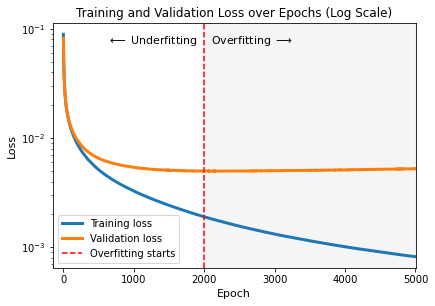
\includegraphics[width=\textwidth]{Pictures/SGD_loss_5000_shaded_dashed.png}
      \caption{Progression of MSE cost}\label{fig:SGD_1}
    \end{minipage}
    \hspace{0.3cm}
    \begin{minipage}[b]{0.465\textwidth}
      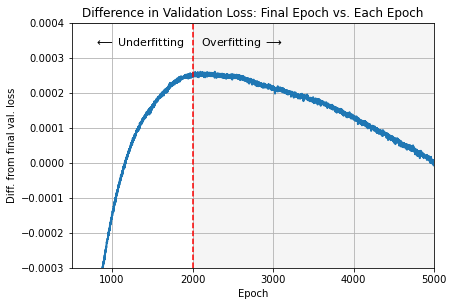
\includegraphics[width=\textwidth]{Pictures/SGD_loss_5000_differences.png}
      \caption{From Underfitting to Overfitting}\label{fig:SGD_2}
    \end{minipage}
\end{figure}\\
Figure \ref{fig:SGD_1} shows a divergence in training and validation loss relatively early on.  During training, the training loss rapidly declines almost to zero as the model continuously optimizes its weights and biases using the training dataset. Meanwhile, the validation loss appears to level off around the 1000th epoch. From this point, it continues to decrease but at a significantly slower pace, until it begins to gradually increase after the 2000th epoch. This trend is further illustrated in Figure \ref{fig:SGD_2}, which displays the difference between the final epoch's validation loss and the validation loss at each preceding epoch. From the 0th to the 2000th epoch, we observe an increasing difference, suggesting an average decrease in validation loss with each epoch, indicative of underfitting, where the model's performance on the validation set can still improve. However, beyond the 2000th epoch, the difference starts to decrease. This suggests that the validation loss increases from the 2000th epoch all the way to the final (5000th) epoch, an indication of overfitting where the model's performance on the validation set deteriorates. One can argue, that it is not feasible to continue training beyond 1000 epochs, even though the validation loss keeps decreasing until the 2000th epoch, since training requires a lot of computer time and any potential improvement after the 1000th epoch can be seen as negligible. Initially, we set the step size to $\tau = 0.01.$ However, as discussed in Subsection \ref{SGD section}, we can increase $\tau$ in an attempt to find minima at which the cost function attains a lower value. For the following series of results, we choose 50 epochs. Although training could theoretically continue beyond this point, computational constraints made further training impractical. Specifically, larger epochs such as 500 and 2000 require several hours to complete a single training and validation loop, making the process time-inefficient. Figure \ref{fig:SGD_FFNN_LR}, plots the decrease in the MSE cost for the training and validation datasets as training progresses and parameters $\theta$ (weights and biases) are updated.\footnote{Refer to Notebook 7, cells 8 and 9, in GitHub \cite{ThesisCode2023}. Change the epoch number in the training loop to 50 for the plot.} This is shown for different step sizes (learning rates) in the set $\{0.01,\text{ }0.05,\text{ }0.1\}.$
\newpage
\begin{figure}[h!]
    \centering
        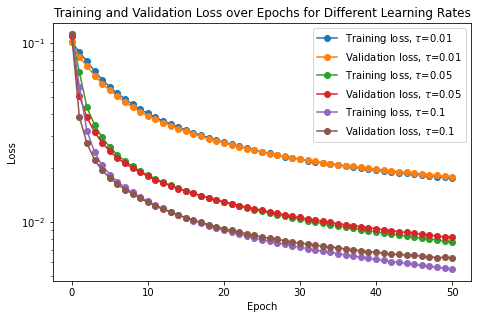
\includegraphics[width=0.47\textwidth]{Pictures/SGD_FFNN_loss_lr_log.png}
    \caption{Progression of MSE cost for various learning rates over 50 epochs}\label{fig:SGD_FFNN_LR}
\end{figure}
As can be observed from the plot (Figure \ref{fig:SGD_FFNN_LR}), within the tested rates $\{0.01,\text{ }0.05,\text{ }0.1\},$ a larger learning rate $\tau$ results in quicker achievement of lower training and validation losses. In other words, the model learns faster with a larger learning rate, within the examined range. This observation is further supported by the fact that the validation loss exceeds the training loss faster for these larger learning rates. 
\subsubsection{Testing the Model}
To evaluate the model's performance after training, we will use the test dataset provided by the MNIST database. This dataset contains 10,000 examples that were not used during training. We will examine how the model's predictions for images in this test dataset change as a result of training. Specifically, we will compare the model's outputs before training (using the initial weights and biases) and after training (using the final weights and biases). We will fix the number of training epochs to 50 for these experiments. Figures \ref{fig:digit_1} and \ref{fig:digit_2} illustrate this comparison for two test images, corresponding to the digits 7 and 4, respectively.
\begin{figure}[h!]
    \centering
    \begin{minipage}[b]{0.40\textwidth}
      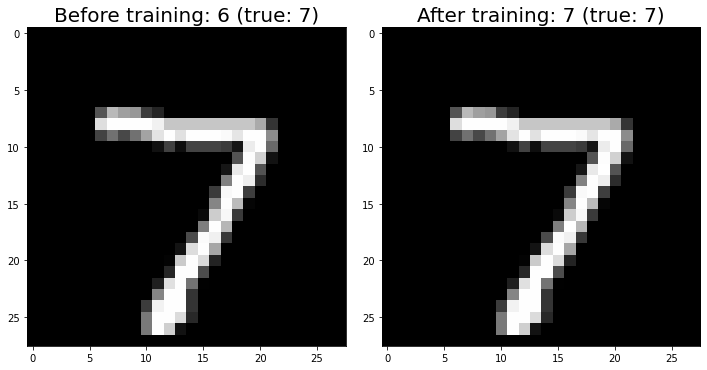
\includegraphics[width=\textwidth]{Pictures/digit_1.png}
      \caption{Example 1}\label{fig:digit_1}
    \end{minipage}
    \hspace{0.3cm}
    \begin{minipage}[b]{0.40\textwidth}
      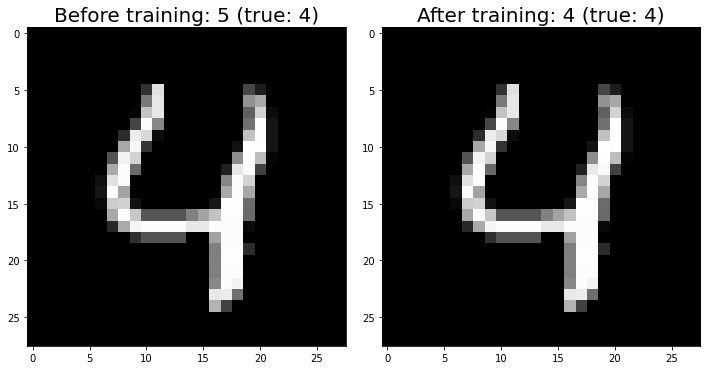
\includegraphics[width=\textwidth]{Pictures/digit_2.png}
      \caption{Example 2}\label{fig:digit_2}
    \end{minipage}
\end{figure}\\
As observed from the figures, prior to training, the model does not correctly predict the digits for both inputs. However, post-training, the model accurately identifies the true digits. This is evident from the fact that the probabilities associated with the 8th and 5th indices in the output vectors (corresponding to the digit classes 7 and 4 respectively, as indices start from 1) are greater than all the other probabilities in these vectors after training. Figure \ref{fig:digit_3} illustrates another comparison of the model's output before and after training for a test image, corresponding to the digit 5. \footnote{Refer to Notebook 7, cells 10-12, in GitHub \cite{ThesisCode2023} to create the images. Any image from the test dataset can be chosen.}
\begin{figure}[h!]
    \centering
        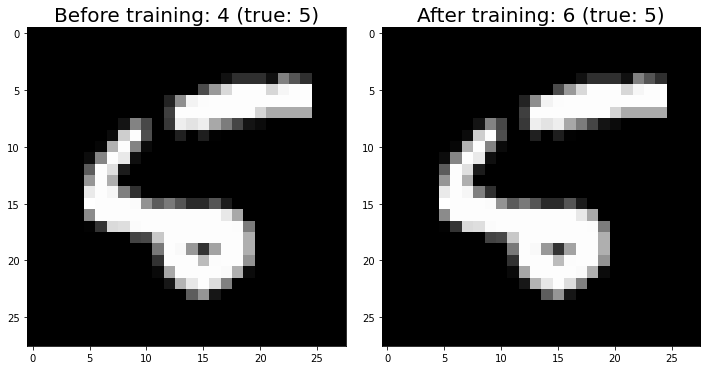
\includegraphics[width=0.40\textwidth]{Pictures/digit_3.png}
    \caption{Example 3}\label{fig:digit_3}
\end{figure}\\
For this example (Figure \ref{fig:digit_3}), the model fails to correctly predict the digit, prior to training and post-training. By looking at the image, even a human observer might struggle to classify it as the digit 5. One could argue that it might actually correspond to the digit 6. In this case, it is possible that the model would need more training to successfully classify the image as a 5. The examples showcased in Figures \ref{fig:digit_1}, \ref{fig:digit_2} and \ref{fig:digit_3} were selected from the 10,000 test images. The performance of the model in classifying these images was evaluated solely based on the model's parameters (weights and biases) before and after the training process. To track how the model's accuracy in classifying the correct digit evolves over the course of the training, it is beneficial to calculate this accuracy at each epoch. Let us define the model's accuracy at the $i$-th epoch, $A^{(i)}$, as the ratio of the number of correct predictions, $C^{(i)}$, to the total number of test images (10,000). A prediction is deemed correct if the model's digit classification of an image matches the known true label of that image. Thus, we can represent the accuracy as follows:
\begin{equation*}\tag{6.4.4.1}
A^{(i)} = \frac{C^{(i)}}{10000} \hspace{0.6cm} \forall i \in \{0,\ldots50\}
\end{equation*}
Here, $A^{(i)}$ is essentially a ratio within the range [0, 1] that depicts the percentage of instances where the model makes a correct prediction. Figures \ref{fig:accuracy_1} and \ref{fig:accuracy_2} illustrate the model's accuracy progression over epochs for different learning rates $\tau,$ specifically for $\tau \in \{0.01,\text{ }0.05,\text{ }0.1\}.$ Figure \ref{fig:accuracy_2} is an amplified version of Figure \ref{fig:accuracy_1}, focusing specifically on the Y-axis range [0.8, 1].\footnote{Refer to Notebook 7, cells 13-15, in GitHub \cite{ThesisCode2023}. Change the epoch number in the training loop to 50 for the plots.}
\begin{figure}[h!]
    \centering
    \begin{minipage}[b]{0.45\textwidth}
      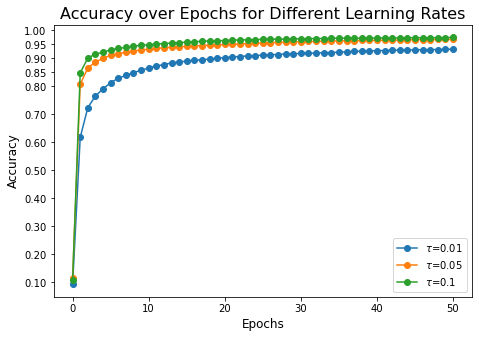
\includegraphics[width=\textwidth]{Pictures/Accuracy_over_epochs_lr.png}
      \caption{Accuracy}\label{fig:accuracy_1}
    \end{minipage}
    \hspace{0.3cm}
    \begin{minipage}[b]{0.45\textwidth}
      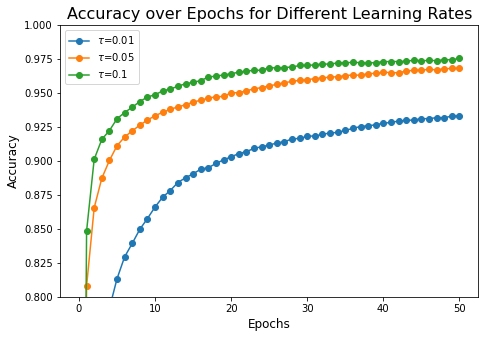
\includegraphics[width=\textwidth]{Pictures/Accuracy_over_epochs_lr_zoom.png}
      \caption{Accuracy (Y-lim: [0.8, 1])}\label{fig:accuracy_2}
    \end{minipage}
\end{figure}\\
As can be seen from Figure \ref{fig:accuracy_1}, the accuracy of the model for all three learning rates (0.01,\text{ }0.05,\text{ }0.1) increases rapidly after just one epoch of training. Subsequently, the accuracy for the learning rate of $0.01$ consistently remains lower than the other two, while the accuracy for the highest learning rate $0.1$ exceeds that of the $0.05$ learning rate, though they remain close. All three accuracy measures show a progression towards higher accuracy. From Figure \ref{fig:accuracy_2}, we observe that at the 50th epoch, the accuracies for all three learning rates exceed $0.925$, indicating that the model's predictions on the test data are correct at least $92.5\%$ of the time in each case.
